\documentclass{article}

\usepackage{graphicx}
\usepackage{amsmath}
\usepackage{amssymb}
\usepackage{caption}

\renewcommand{\figurename}{Figura}

\begin{document}

\begin{flushleft}
    \LARGE Banjercito \\[6pt]
    \Large Diplomado en Ciencia de Datos
\end{flushleft}

\vfill

\begin{flushleft}
    \LARGE \textbf{Tarea 501} \\[12pt]
    \LARGE Módulo V | Semana 1 \\[24pt]
\end{flushleft}

\vfil

\begin{flushleft}
    Alan Badillo Salas \\[12pt]
    Noviembre 2024 \\[24pt]
\end{flushleft}

\vfill

\section*{Introducción}
El Diplomado en Ciencia de Datos ha llegado a su quinto módulo titulado "\textit{Deep Learning}". En este módulo revisaremos a profundidad las redes neuronales generales, recurrentes y convolutivas para resolver problemas generales y particulares de forma automática, mejorando así la predicción y pronóstico en los análisis y casos de estudio relacionados.
\\[12pt]
En la semana 1 hemos hecho un repaso sobre los temas más importantes de los módulos anteriores, partiendo del uso de Python, Numpy y Pandas, así como la probabilidad y estadística bayesiana y de los modelos de Regresión y Clasificación de Machine Learning. También se introdujo el concepto de \textit{Perceptrón} y su aplicación para predecir un objetivo a través de sus características.
\\[12pt]
En esta tarea se reforzarán las habilidades para hacer un análisis de interés simple con Excel y Python.

\clearpage

\section*{Tarea 501 | Tabla de Interés simple}

Una financiera requiere calcular el interés simple de una serie de montos y poder sustituir la tasa de interés en cualquier momento.
\\[12pt]
Genera una hoja de Excel que contenga los siguientes montos:

\begin{table}[h!]
\centering
\begin{tabular}{|c|c|}
\hline
\textbf{Número} & \textbf{Monto (USD)} \\ \hline
1  & 100.00   \\ \hline
2  & 250.50   \\ \hline
3  & 375.25   \\ \hline
4  & 480.75   \\ \hline
5  & 520.00   \\ \hline
6  & 630.40   \\ \hline
7  & 745.30   \\ \hline
8  & 890.90   \\ \hline
9  & 935.60   \\ \hline
10 & 1020.80  \\ \hline
11 & 1135.00  \\ \hline
12 & 1250.75  \\ \hline
13 & 1375.90  \\ \hline
14 & 1420.60  \\ \hline
15 & 1555.25  \\ \hline
16 & 1670.50  \\ \hline
17 & 1805.75  \\ \hline
18 & 1920.40  \\ \hline
19 & 2050.00  \\ \hline
20 & 2185.50  \\ \hline
\end{tabular}
\caption{Tabla de montos de dinero}
\label{tab:montos_dinero}
\end{table}
\hfill\\
Calcula el interés simple anual usando una tasa anual del 8\%. Recalcula el interés usando una tasa de 13\%.
\\[12pt]
Reporta la suma del interés anual generado con la tasa del 8\% y la suma con la tasa del 13\%.
\\[12pt]
Genera una gráfica de pastel que compare la suma de intereses al 8\% y 13\%. ¿Cuál es el porcentaje de la suma de intereses al 8\% respecto al del 13\%?
\\[12pt]
En la Figura \ref{fig:p501a} se muestran los resultados esperados en Excel, para activar las etiquetas de la gráfica se deben agregar en \textit{Diseño de gráfico / Agregar elemento de gráfico / Etiquetas de datos}.
\\[12pt]
\begin{figure}[h]
    \centering
    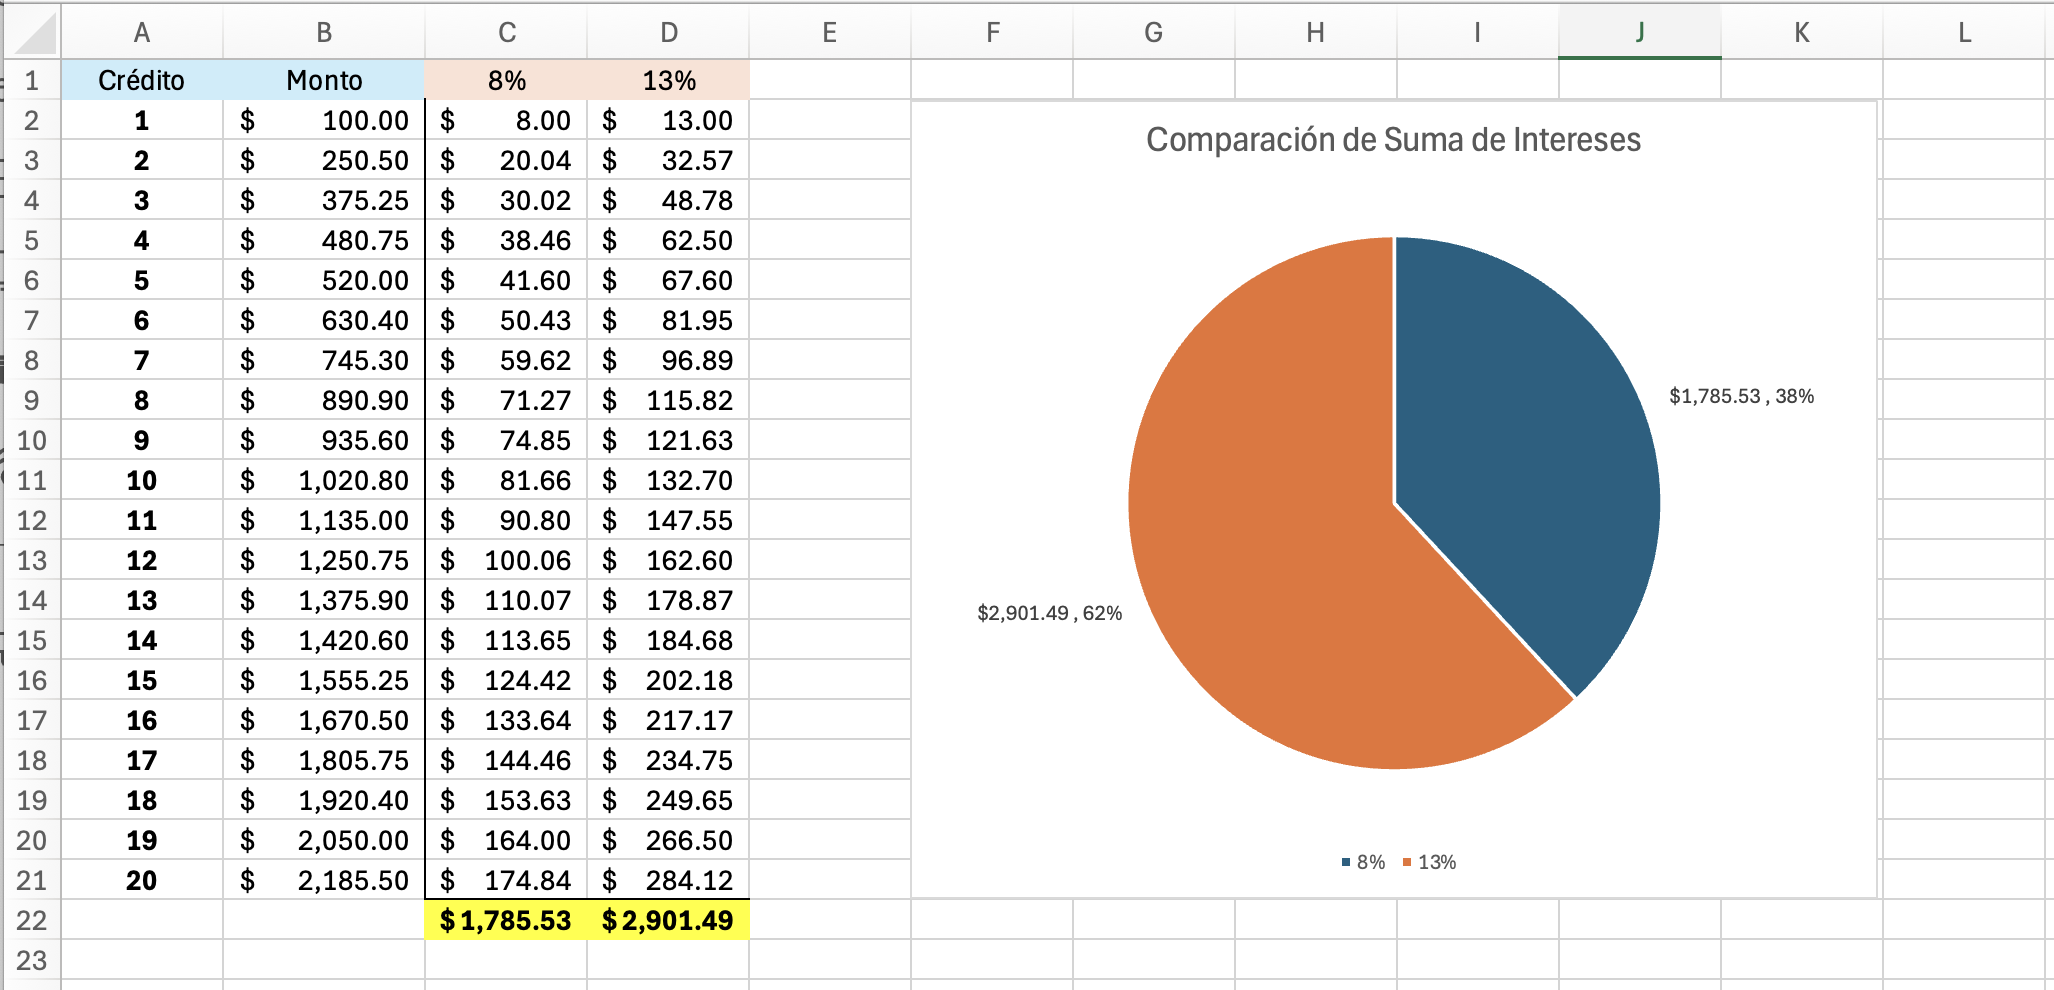
\includegraphics[width=0.8\textwidth]{figures/p501a.png}
    \captionsetup{width=\textwidth}
    \caption{Resulados esperados en Excel}
    \label{fig:p501a}
\end{figure}
\\[12pt]
Exporta la tabla de montos en un CSV llamado \textit{montos.csv} o usa directamente el archivo de Excel para procesarlo con python.
\\[12pt]
Sigue los pasos del \textit{script} para generar el reporte de montos, intenta ejecutar línea por línea en una celda y hacer las anotaciones necesarias.
\begin{verbatim}
    # Importamos la librería de pandas
    import pandas

    # Cargamos los datos del archivo de excel p501.xlsx
    # en el DataFrame de pandas llamado "montos"
    # para la Hoja1
    # limitado las primeras 20 filas
    # sobre las columnas A y 20
    montos = pandas.read_excel("/content/p501.xlsx", 
                            sheet_name="Hoja1", 
                            nrows=20, usecols="A:B")

    # Mostramos la tabla de montos
    montos

    # Calculamos la suma de los intereses al 8%
    suma_8p = montos["8%"].sum()
    # Calculamos la suma de los intereses al 13%
    suma_13p = montos["13%"].sum()

    # Importamos la sublibrería de graficación pyplot
    import matplotlib.pyplot as pyplot

    # Graficamos la suma al 8% respecto la suma al 13%
    # agregamos etiquetas y porcentajes
    pyplot.pie([suma_8p, suma_13p], 
            labels=[f"${suma_8p:.2f}, 8%", 
                    f"${suma_13p:.2f}, 13%"], 
            autopct="%.2f%%")
    # Guardamos la gráfica como p501.png
    pyplot.savefig("p501.png")
    # Mostramos la gráfica
    pyplot.show()
    pyplot.show()
\end{verbatim}
En la Figura \ref{fig:p501b} observamos la gráfica de pastel que compara la suma de intereses al 8\% y 13\% generada en python por matplotlib.
\begin{figure}[h]
    \centering
    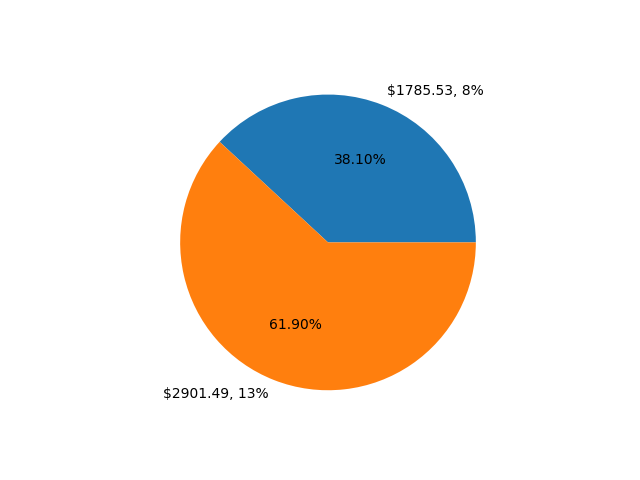
\includegraphics[width=0.8\textwidth]{figures/p501b.png}
    \captionsetup{width=\textwidth}
    \caption{Gráfica de pastel generada por Matplotlib}
    \label{fig:p501b}
\end{figure}
\\[12pt]
Responda las siguientes preguntas y anote sus conclusiones:
\begin{enumerate}
    \item ¿Qué significa que significa que \$1,785.53 sea el 38.10\% y \$2,901.49 sea el 61.90\%?
    \item Si la financiera decidiera aumentar 1\% la tasa de interés anual (considerando el 8\% actual), ¿Cuánto ganaría sobre los montos actuales y qué porcentaje de incremento representaría respecto al del 8\%?
    \item Si se perdiera el crédito por el monto de \$1,670.50, ¿Qué porcentaje debería subir la tasa de interés para no tener pérdidas?
\end{enumerate}

\end{document}